\section{考察}
基礎実験の結果より通常指及び半球型指で把持中には荷重を検出し解放後は荷重を検出しなくなったことからグリッパの把持状態の検出に成功した.\par
荷重実験の結果より通常指は把持力の増加に伴う荷重の増加を検出できた.しかし右指と比べて左指は計測値が小さくなっている.これは左指と対象物との接触位置がセンサ部と離れ,十分に力が伝わらなかったからであると考えられる.\\
一方半球型指は球と円筒に関して計測値の左右差はほぼ無くセンサ部に十分力が伝わっている.これは半球型指が押されると半球の凸部に荷重が集中したためであると考察する.ボトルに関しては球と円筒に比べて計測値が小さく増減も見られない.把持の様子を\refig{cap_grasp}に示すように把持時に半球が上下非対称に変形し凸面の位置がずれセンサ部に十分に力が伝わらなかったと考える.\par
引張実験より\reftab{e3}に通常指と半球型指の対象物ごとの静止摩擦力の差を示す.この表より通常指の方が半球型指よりすべての把持対象物で大きく把持時の拘束力が優れていることがわかる.この理由は通常指のほうが平均的に柔軟部が厚く対象物を包む接触面積が大きくなり摩擦力が増加したからであると考えられる.今後の課題として半球型指の把持部をより厚くし拘束力を向上が求められる.

\begin{figure}[htbp]
\centering
\subfloat[把持の様子]{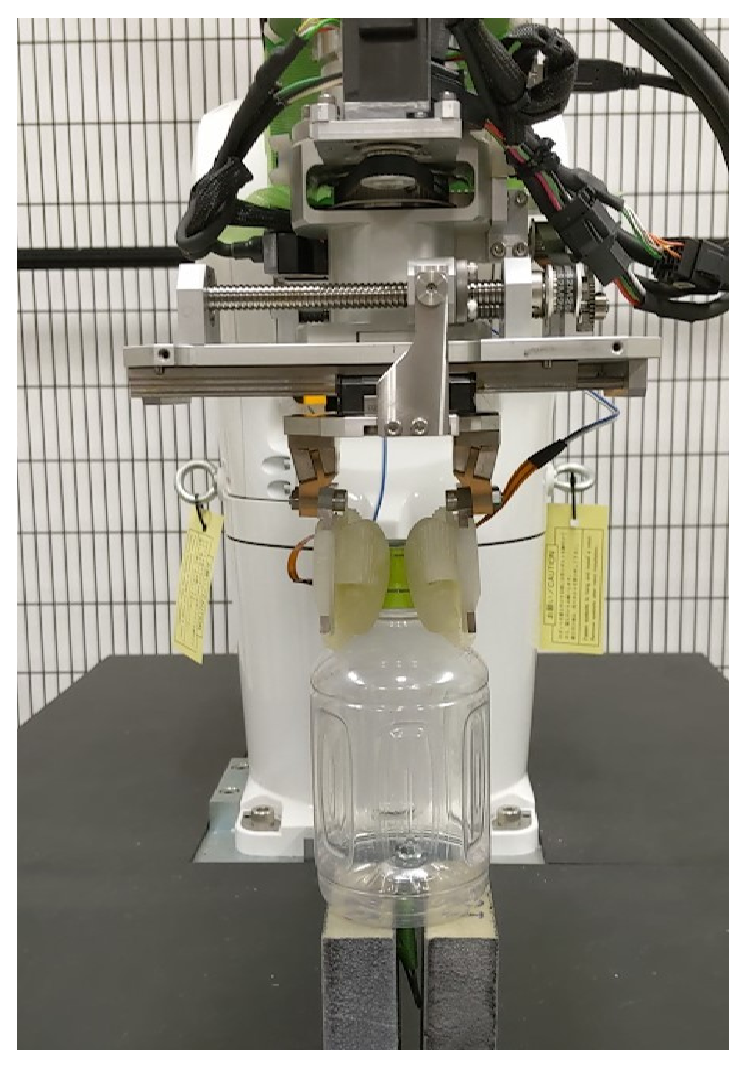
\includegraphics[scale=0.4]{../fig/eps/cap_grasp.eps}}
\hspace{5mm}
\subfloat[拡大]{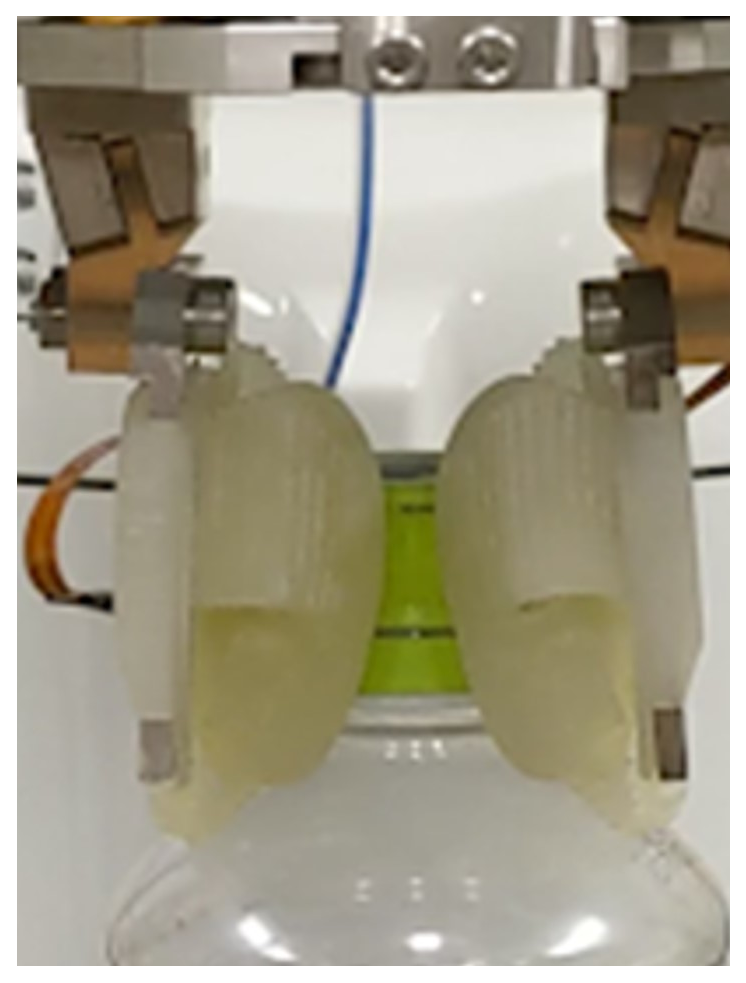
\includegraphics[scale=0.4]{../fig/eps/cap_grasp2.eps}}
\hspace{5mm}\\
\caption{半球型指でのボトル把持の様子}
\label{fig::cap_grasp}
\end{figure}

\begin{table}[t]
    \caption{静止摩擦力比較}
   \label{tab::e3}
   %\scalebox{3}[1.5]
   \centering
   \begin{tabular}{|c||c|c|c|} \hline
   Force[N]   &Ball     &Cylinder      &Bottle    \\ \hline \hline
        15 & 5.63 & 10.68 & 12.56   \\ \hline
        18  & 4.54 & 6.71  & 13.99    \\ \hline
        21  & 7.44 & 11.76  & 10.77    \\ \hline
		24  & 4.63 & 13.46  & 8.97   \\ \hline
		27  & 7.96 & 10.58  & 13.01   \\ \hline			
		30 & 1.44 & 14.96  & 8.92   \\ \hline
		Average  & 5.27 & 11.36  & 11.37   \\ \hline
		 \end{tabular}
\end{table}

